% Completa los datos convenientemente en las zonas marcadas con TODO

\documentclass{beamer}
%PARA VISUALIZAR PRESENTACIONN CON NOTAS USAR VISUALIZADOR "pdfpc":
%Para ver las notas, el cronometro y siguente diapo:
% pdfpc --notes=right slides.pdf
% "tecla p": para pausar el cronometro
\mode<presentation> {
  \usetheme{CambridgeUS}
  \usecolortheme{crane} % color naranja
}
\setbeamercolor{titlelike}{parent=structure,bg=yellow!85!orange} % Cambia el color de la caja del título de la página inicial

\setbeamertemplate{navigation symbols}{} % ocultar iconos de navegación
\setbeamerfont{subsection in toc}{size=\small} % reducir tamaño en TOC
\setbeamerfont{date}{size=\tiny}
\usepackage[spanish]{babel}
\usepackage[utf8]{inputenc}
\usepackage{graphicx}
\usepackage{booktabs}
\usepackage{hyperref}
\usepackage{multicol}
\usepackage{pgfpages}
\usepackage{listings}
\usepackage{multimedia}
\usepackage[export]{adjustbox}
\usepackage{outlines} % Para poner bullets tabulados (\1 \2 \3 ...) y no items

\usepackage{amsmath}
\usepackage{physics}  % Paquete necesario para \abs{}

\usepackage{array,tabularx} % para tabular leyenda de ecuaciones
\newenvironment{conditions*} % entorno de "leyenda de ecuación"
  {\par\vspace{\abovedisplayskip}\noindent
   \tabularx{\columnwidth}{>{$}l<{$} @{\ : } >{\raggedright\arraybackslash}X}}
  {\endtabularx\par\vspace{\belowdisplayskip}}
  
% USO DE NOTAS
\setbeameroption{hide notes} % Para mostrar u ocultar (hide/show)
%\setbeameroption{show only notes} % Mostrar solo las notas
%\setbeameroption{show notes on second screen=right} % Mostrar notas en otra pantalla
\setbeamertemplate{note page}{ % asi solo muestro el texto de las notas
  \insertnote%
}

%========= TODO: datos internos del documento
\hypersetup{
	pdftitle={Defensa de trabajo de fin de grado de Julia López Augusto},
	pdfauthor={Julia López Augusto},
	pdfsubject={Robot de bajo coste para el mantenimiento de carreteras},
	pdfkeywords={teaching, robotics, vision, sensors, actuators, raspberry},
	pdfproducer={pdfLaTeX},
  colorlinks=true,
  linkcolor=blue
}
%=========

%========= TODO: diapositiva de portada
\title[Robot de bajo coste para el mantenimiento]{Robot de bajo coste para \newline el mantenimiento de carreteras} % El título reducido aparece en la parte inferior de todas las diapositivas
                                         % El título completo aparece solo en la diapositiva de portada
\author[Julia López Augusto]{Julia López Augusto}
\institute[URJC]
{
\textit{\href{mailto:escribe.tu@correo.es}{\color{blue}{\underline{j.lopeza.2020@alumnos.urjc.es}}}}\\
\vspace{0.5cm}

\includegraphics[width=3cm]{figs/logo-urjc}\\
\vspace{1cm}
Trabajo Fin de Grado
}
\date{18 de diciembre de 2024}
%=========

%========= COMIENZO DEL DOCUMENTO
\begin{document}

%========= Portada inicial con notas
\begin{frame}[plain] % plain: quita header y footer
\large{\titlepage}
\note[item]{En esta presentación voy a hablar sobre...}
\note[item]{En primer lugar...}
\end{frame}

%========= Licencia
\begin{frame}
% Este diseño se corresponde con la licencia CC-BY-NC-SA.
% Por supuesto, puedes poner la licencia que mejor se adapte al propósito de tu trabajo.
% Recuerda que, si no se especifica ninguna licencia, esta -como cualquier creación artística- pasaría a estar licenciada con todos los derechos reservados (copyright).

\cleardoublepage

\begin{figure}
 \ \ \ \ 
\includegraphics[width=0.25\linewidth]{figs/by-nc-sa.png}
 \label{fig:cc} 
 \end{figure}

\

\

\

\noindent
Este trabajo se distribuye bajo los términos de la licencia internacional \href{http://creativecommons.org/licenses/by-nc-sa/4.0/}{CC BY-NC-SA International License} (Creative Commons AttributionNonCommercial-ShareAlike 4.0). Usted es libre de \textit{(a) compartir}: copiar y redistribuir el material en cualquier medio o formato; y \textit{(b) adaptar}: remezclar, transformar y crear a partir del material. El licenciador no puede revocar estas libertades mientras cumpla con los términos de la licencia:

\begin{itemize}
\item \textit{Atribución}. Usted debe dar crédito de manera adecuada, brindar un enlace a la licencia, e indicar si se han realizado cambios. Puede hacerlo en cualquier forma razonable, pero no de forma tal que sugiera que usted o su uso tienen el apoyo de la licenciante.
\item \textit{No comercial}. Usted no puede hacer uso del material con propósitos comerciales.
\item \textit{Compartir igual}. Si remezcla, transforma o crea a partir del material, debe distribuir su contribución bajo la la misma licencia del original.
\end{itemize}

\begin{flushright}
		\vspace{7.0 cm}
		\emph{Documento de} \textbf{Julia López Augusto}. % TODO: pon aquí tu nombre cuando hagas el documento
\end{flushright}


\end{frame}

%========= Índice o tabla de contenidos (TOC)
\begin{frame}
% Título del índice
\frametitle{Contenidos}
%\begin{multicols}{2} % si tengo muchas secciones, lo parte en dos columnas
  \tableofcontents[hideallsubsections] % no muestra subsecciones
%\end{multicols}
\note[item]{La presentación esta dividida en cuatro partes.}
\end{frame}

%============================= Introducción =========================================
%========= Diapositiva "vacía" de comienzo de sección:
\section*{}
\begin{frame}{}
  \centering \Huge
  \emph{Introducción}
\note[item]{Comencemos con la introducción.}
\end{frame}

% Título en azul (pequeñito) 
\section{Introducción}
% Título en azul (pequeñito) 
%\subsection{Robótica}
%========= Diapositiva con imágenes:
\begin{frame}
\frametitle{Robots de campo}
\begin{figure}
\begin{table}[htbp]
	\centering
	\begin{tabular}{cc}
		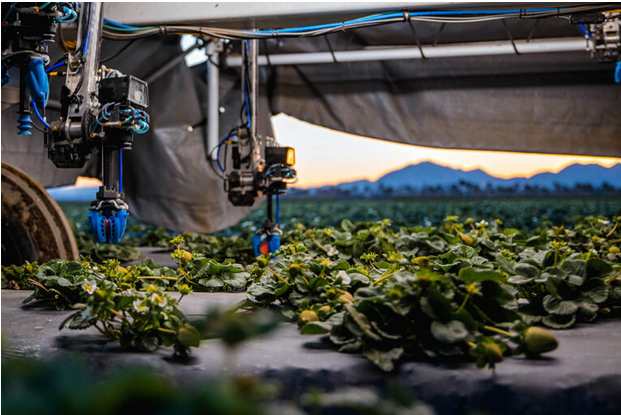
\includegraphics[width=0.3\textwidth, valign=m]{figs/strawberry.png} & 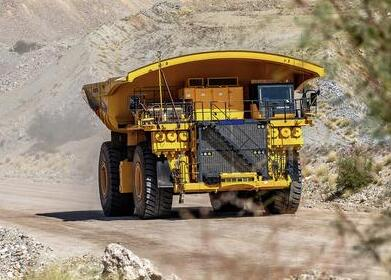
\includegraphics[width=0.3\textwidth, valign=m]{figs/komatsu.jpeg} \\
		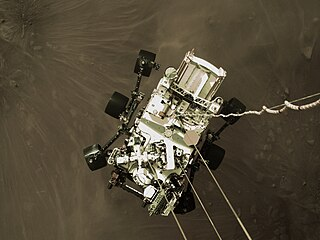
\includegraphics[width=0.3\textwidth, valign=m]{figs/perseverance.jpg} & 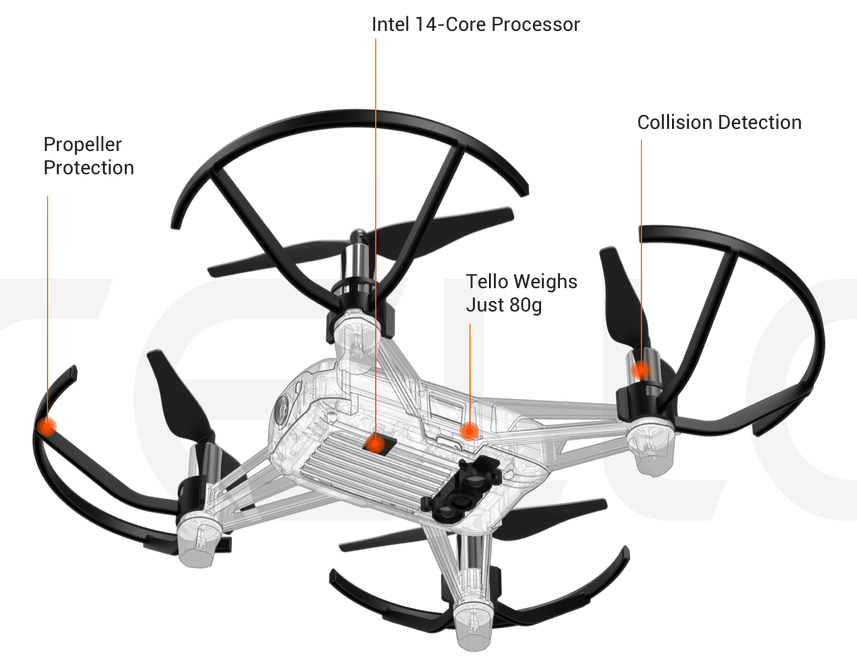
\includegraphics[width=0.3\textwidth, valign=m]{figs/tello.png} 
	\end{tabular}
\end{table}
\end{figure}
\end{frame}

%===================================================================================
%============================= Objetivos ===========================================
\section*{}
\begin{frame}{}
  \centering \Huge
  \emph{Objetivos}
\note[item]{Pasemos ahora a comentar los objetivos que nos hemos enfrentado con este trabajo.}
\end{frame}

\section{Objetivos}
\begin{frame}
	\frametitle{Descripción del problema}
	% Parte superior con 2 imágenes centradas
	\begin{center}
		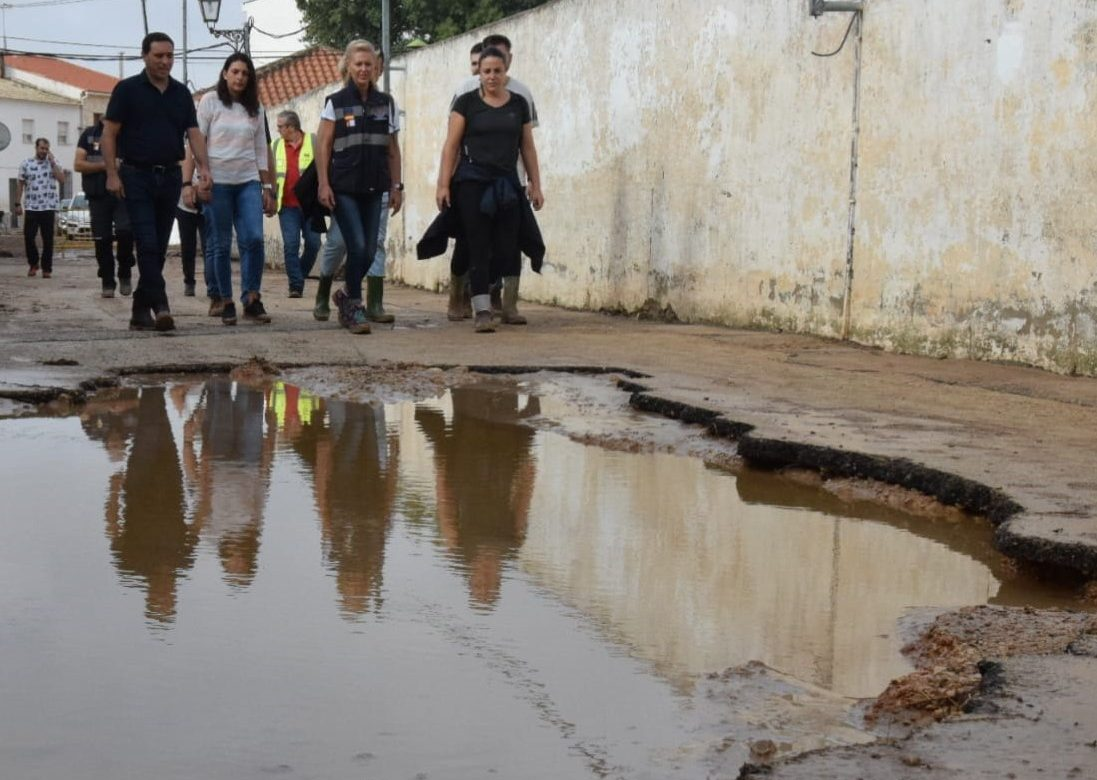
\includegraphics[width=0.3\textwidth]{figs/dana.jpg} \hspace{0.5cm}
		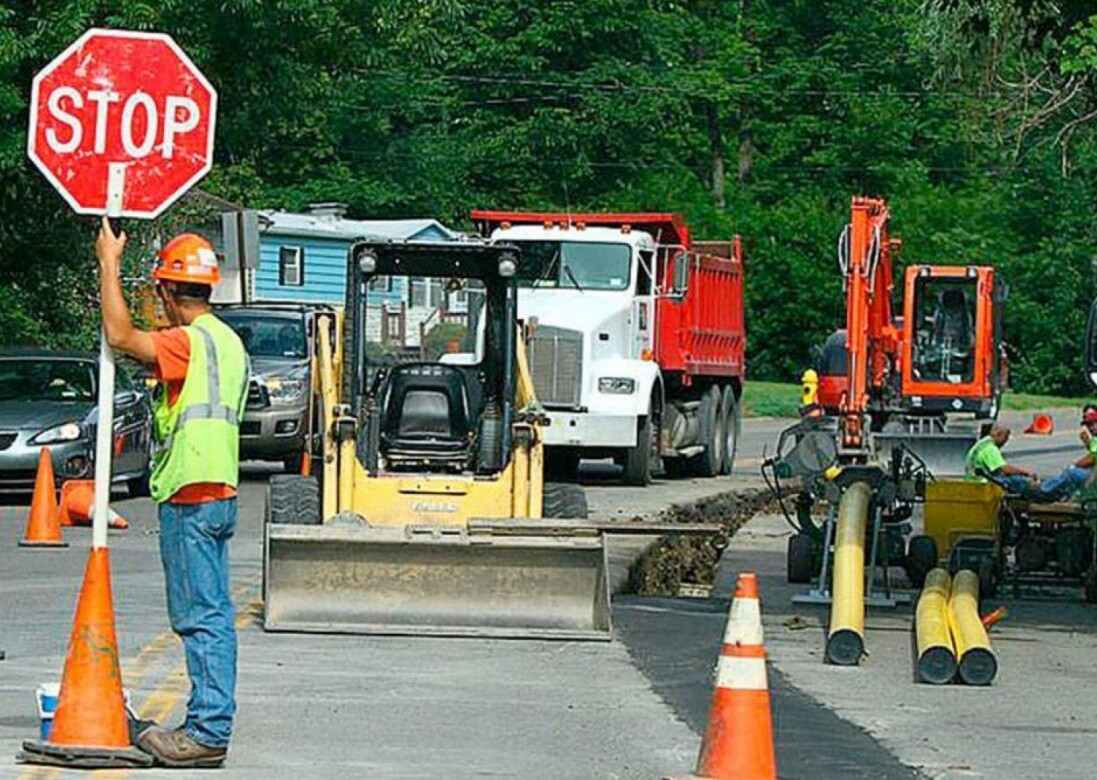
\includegraphics[width=0.3\textwidth]{figs/seguridad.jpg}
	\end{center}
	
	\vspace{0.5cm}  % Espacio entre las imágenes de arriba y las de abajo
	
	% Parte inferior con 1 imagen a la izquierda y 2 imágenes una debajo de otra a la derecha
	\begin{center}
	\begin{columns}
		% Columna izquierda
		\begin{column}{0.5\textwidth}
			\raggedleft
			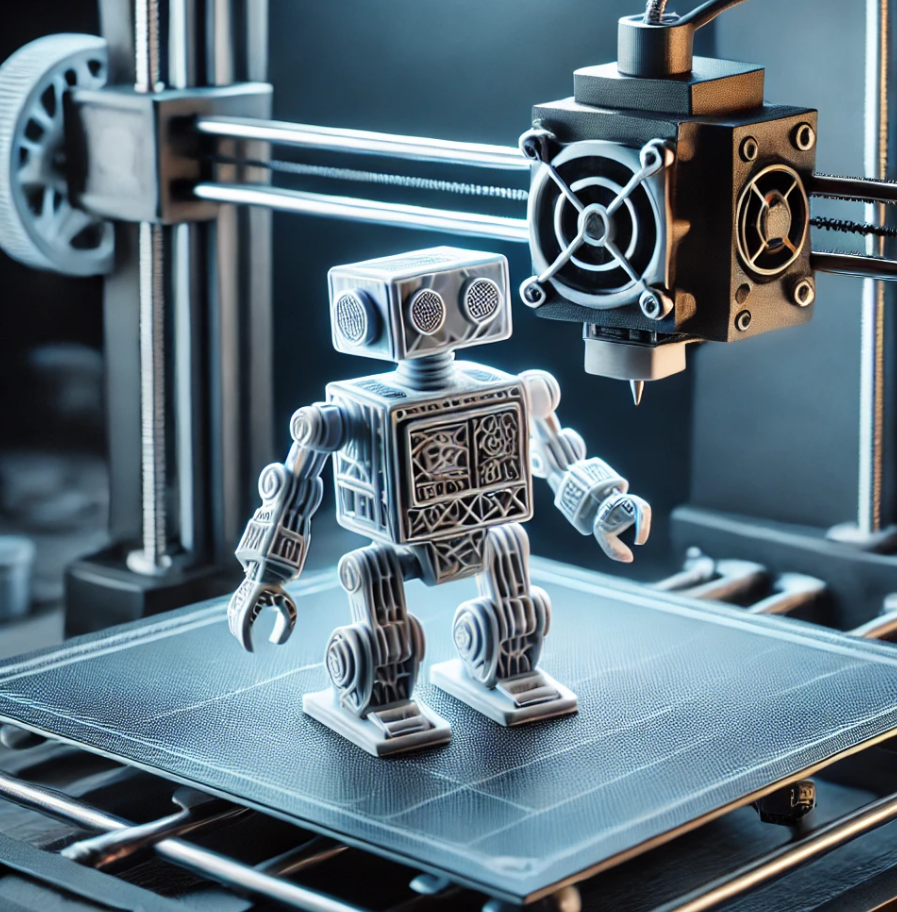
\includegraphics[width=0.55\textwidth]{figs/impresion.png} \\[5pt]
		\end{column} \hspace{0.5cm}
		% Columna derecha
		\begin{column}{0.5\textwidth}
			\raggedright
			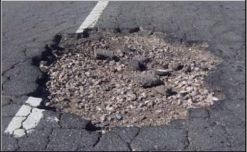
\includegraphics[width=0.4\textwidth]{figs/bache.png} \\[5pt]
			
\includegraphics[width=0.4\textwidth]{figs/interfaceweb.png} \\[5pt]
		\end{column}
	\end{columns}
	\end{center}
\end{frame}


\begin{frame}
\frametitle{Requisitos}
\begin{enumerate}
	\item Coste inferior a 250€.
	\item Piezas impresas en una impresora convencional.
	\item Ubuntu como sistema operativo.
	\item No se requiere tarjeta gráfica dedicada para entrenar modelos.
	\item Modelos adaptados a las limitaciones hardware.
	\item Integración con ROS 2.
\end{enumerate}
\end{frame}

\begin{frame}
	\frametitle{Metodología}
	\begin{figure}
		\centering
		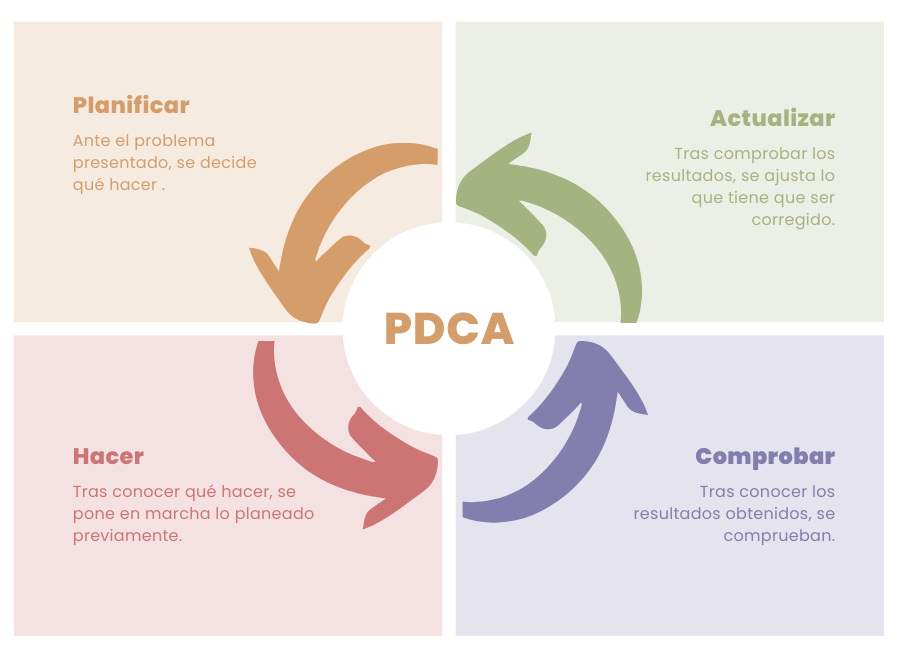
\includegraphics[width=10cm]{figs/PDCA.png}
	\end{figure}
	
\end{frame}

\begin{frame}
	\frametitle{Plan de trabajo}
	\begin{columns}
		% Columna izquierda
		\begin{column}{0.40\textwidth}
			\centering
			
\includegraphics[width=0.8\textwidth]{figs/github.png} \\[5pt]
			\href{https://github.com/RoboticsURJC/tfg-jlopez}{Repositorio}
		\end{column}
		% Columna derecha
		 \begin{column}{0.5\textwidth}
			\centering
			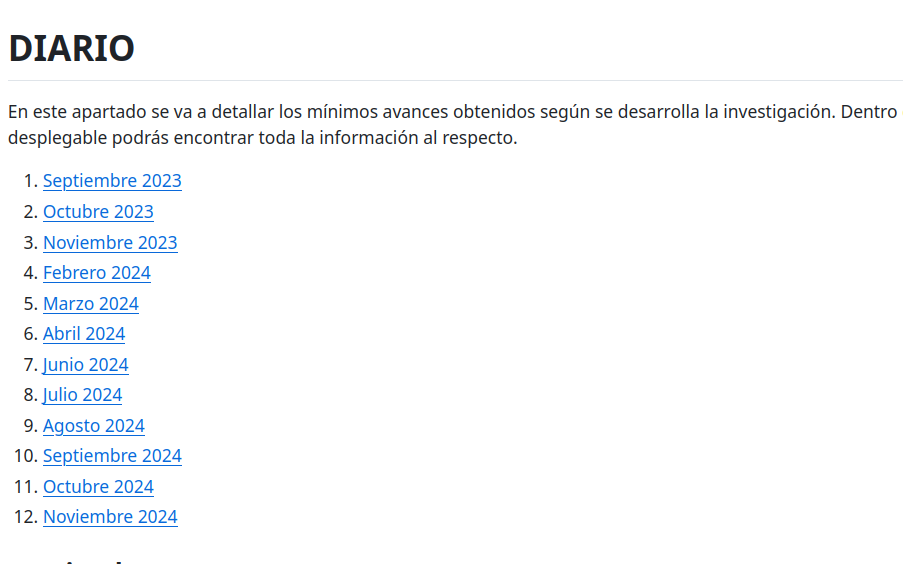
\includegraphics[width=0.8\textwidth]{figs/diario.png} \\[5pt]
			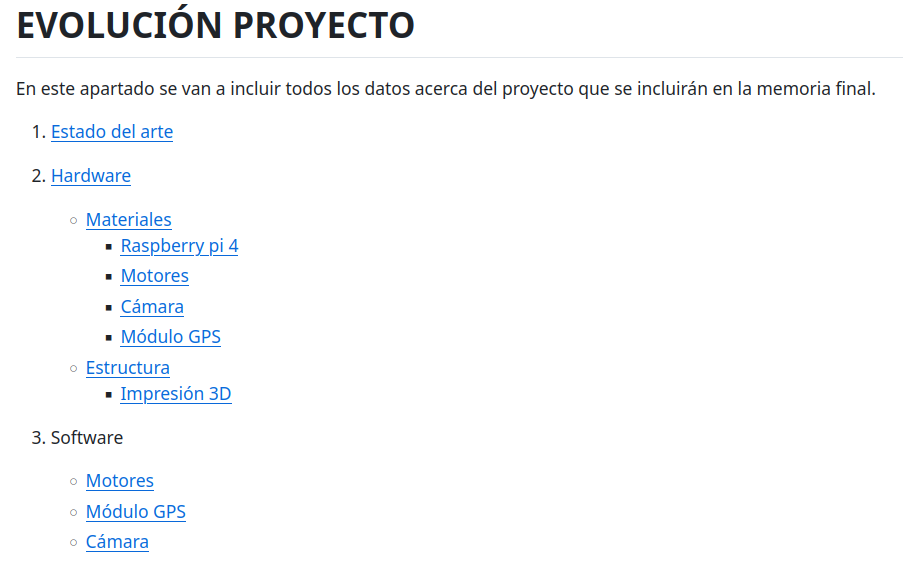
\includegraphics[width=0.8\textwidth]{figs/evo.png} \\[5pt]
			\href{https://github.com/RoboticsURJC/tfg-jlopez/wiki}{Wiki}
		\end{column}
	\end{columns}
\end{frame}

%===================================================================================

%================= Plataforma de desarrollo ========================================
\section*{}
\begin{frame}{}
	\centering \Huge
	\emph{Plataforma de desarrollo}
	\note[item]{Pasemos ahora a comentar los objetivos que nos hemos enfrentado con este trabajo.}
\end{frame}

\section{Plataforma de desarrollo}
\begin{frame}
\frametitle{Hardware}
\begin{figure}
	\centering
	\begin{tabular}{ccc} % 3 columnas
		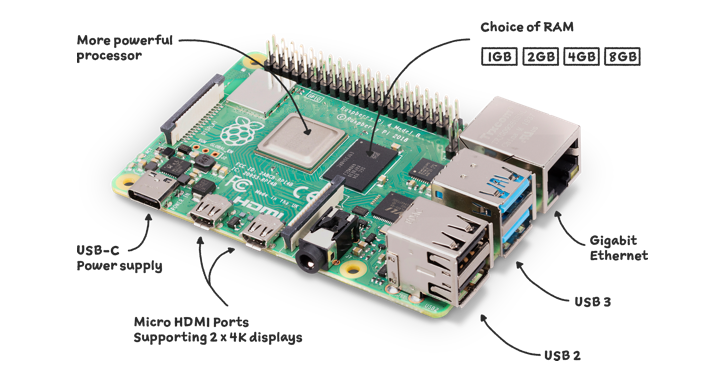
\includegraphics[width=0.2\textwidth]{figs/raspberrypi4.png} & 
		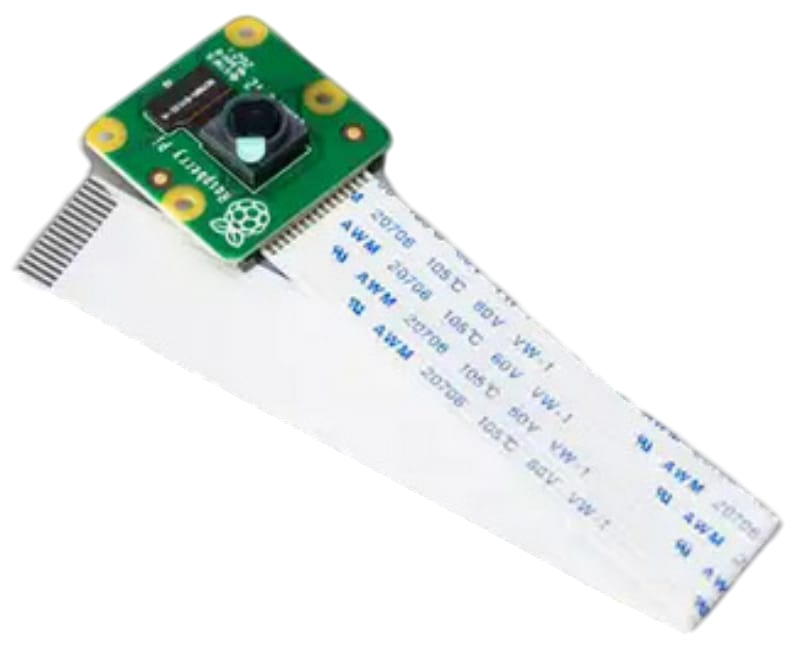
\includegraphics[width=0.15\textwidth]{figs/camera.png} & 
		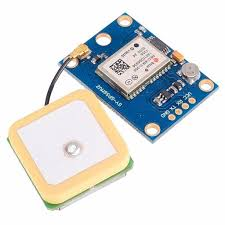
\includegraphics[width=0.15\textwidth]{figs/GPSNEO6MV2.jpeg} \\
		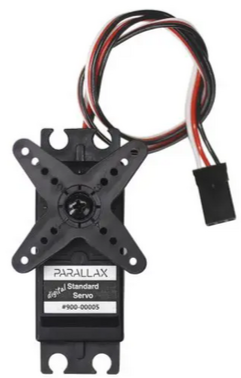
\includegraphics[width=0.1\textwidth]{figs/parallax.png} & 
		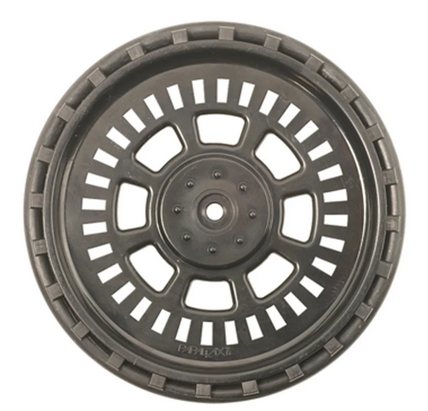
\includegraphics[width=0.15\textwidth]{figs/wheel.png} & 
		\includegraphics[width=0.15\textwidth]{figs/wheel2.png} \\
		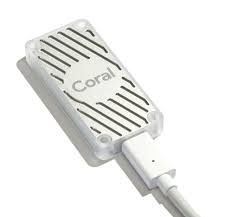
\includegraphics[width=0.15\textwidth]{figs/googlecoral.png} & 
		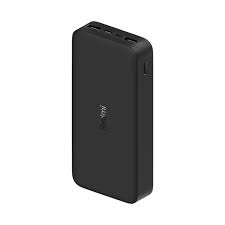
\includegraphics[width=0.15\textwidth]{figs/powerbank.png} & 
		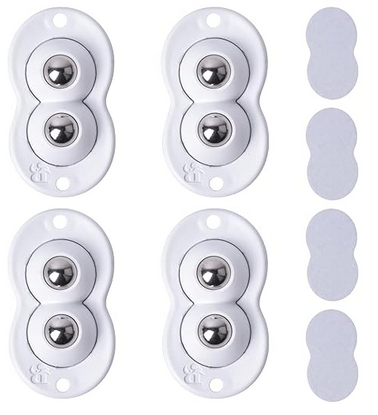
\includegraphics[width=0.1\textwidth]{figs/ruedaloca.png} \\
		\multicolumn{3}{c}{
			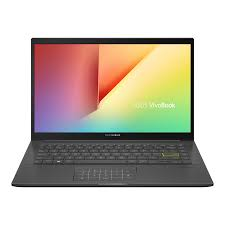
\includegraphics[width=0.15\textwidth]{figs/ordenador.png}
		}
	\end{tabular}
\end{figure}
\end{frame}

\begin{frame}
	\frametitle{Software}
	\begin{figure}
	\centering
	\begin{tabular}{ccc} % 3 columnas
		
\includegraphics[width=0.14\textwidth]{figs/ubuntu.png} & 
		
\includegraphics[width=0.14\textwidth]{figs/freecad.png} & 
		
\includegraphics[width=0.14\textwidth]{figs/python.png} \\
		
\includegraphics[width=0.14\textwidth]{figs/opencv.png} & 
		
\includegraphics[width=0.14\textwidth]{figs/humble.png} & 
		
\includegraphics[width=0.14\textwidth]{figs/foxy.png} \\
		
\includegraphics[width=0.14\textwidth]{figs/gazebo.png} & 
		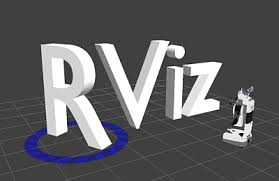
\includegraphics[width=0.14\textwidth]{figs/rviz.png} & 
		
\includegraphics[width=0.14\textwidth]{figs/googlecolab.png} \\
		
\includegraphics[width=0.14\textwidth]{figs/yolov8.png} &
		
\includegraphics[width=0.14\textwidth]{figs/tflite.png} &
		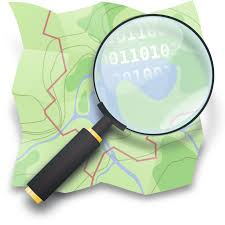
\includegraphics[width=0.14\textwidth]{figs/osm.png}

	\end{tabular}
	\end{figure}	
\end{frame}


%===================================================================================
%============= Diseño y construcción del robot =====================================
\section*{}
\begin{frame}{}
	\centering \Huge
	\emph{Diseño y construcción del robot}
	\note[item]{Pasemos ahora a comentar los objetivos que nos hemos enfrentado con este trabajo.}
\end{frame}

\section{Diseño y construcción del robot}
\begin{frame}
	\frametitle{Geometría del robot}

	\begin{columns}
		% Columna izquierda
		\begin{column}{0.50\textwidth}
			\centering
			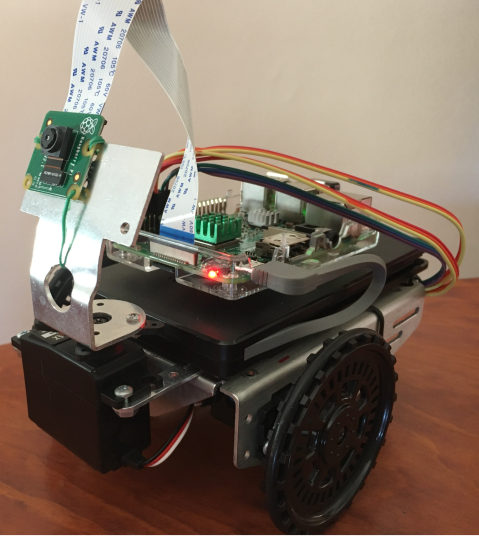
\includegraphics[width=0.85\textwidth]{figs/Original.png} \\[5pt]
			%\caption{Descripción de la imagen 1}
		\end{column}
		% Columna derecha
		\begin{column}{0.5\textwidth}
			\centering
			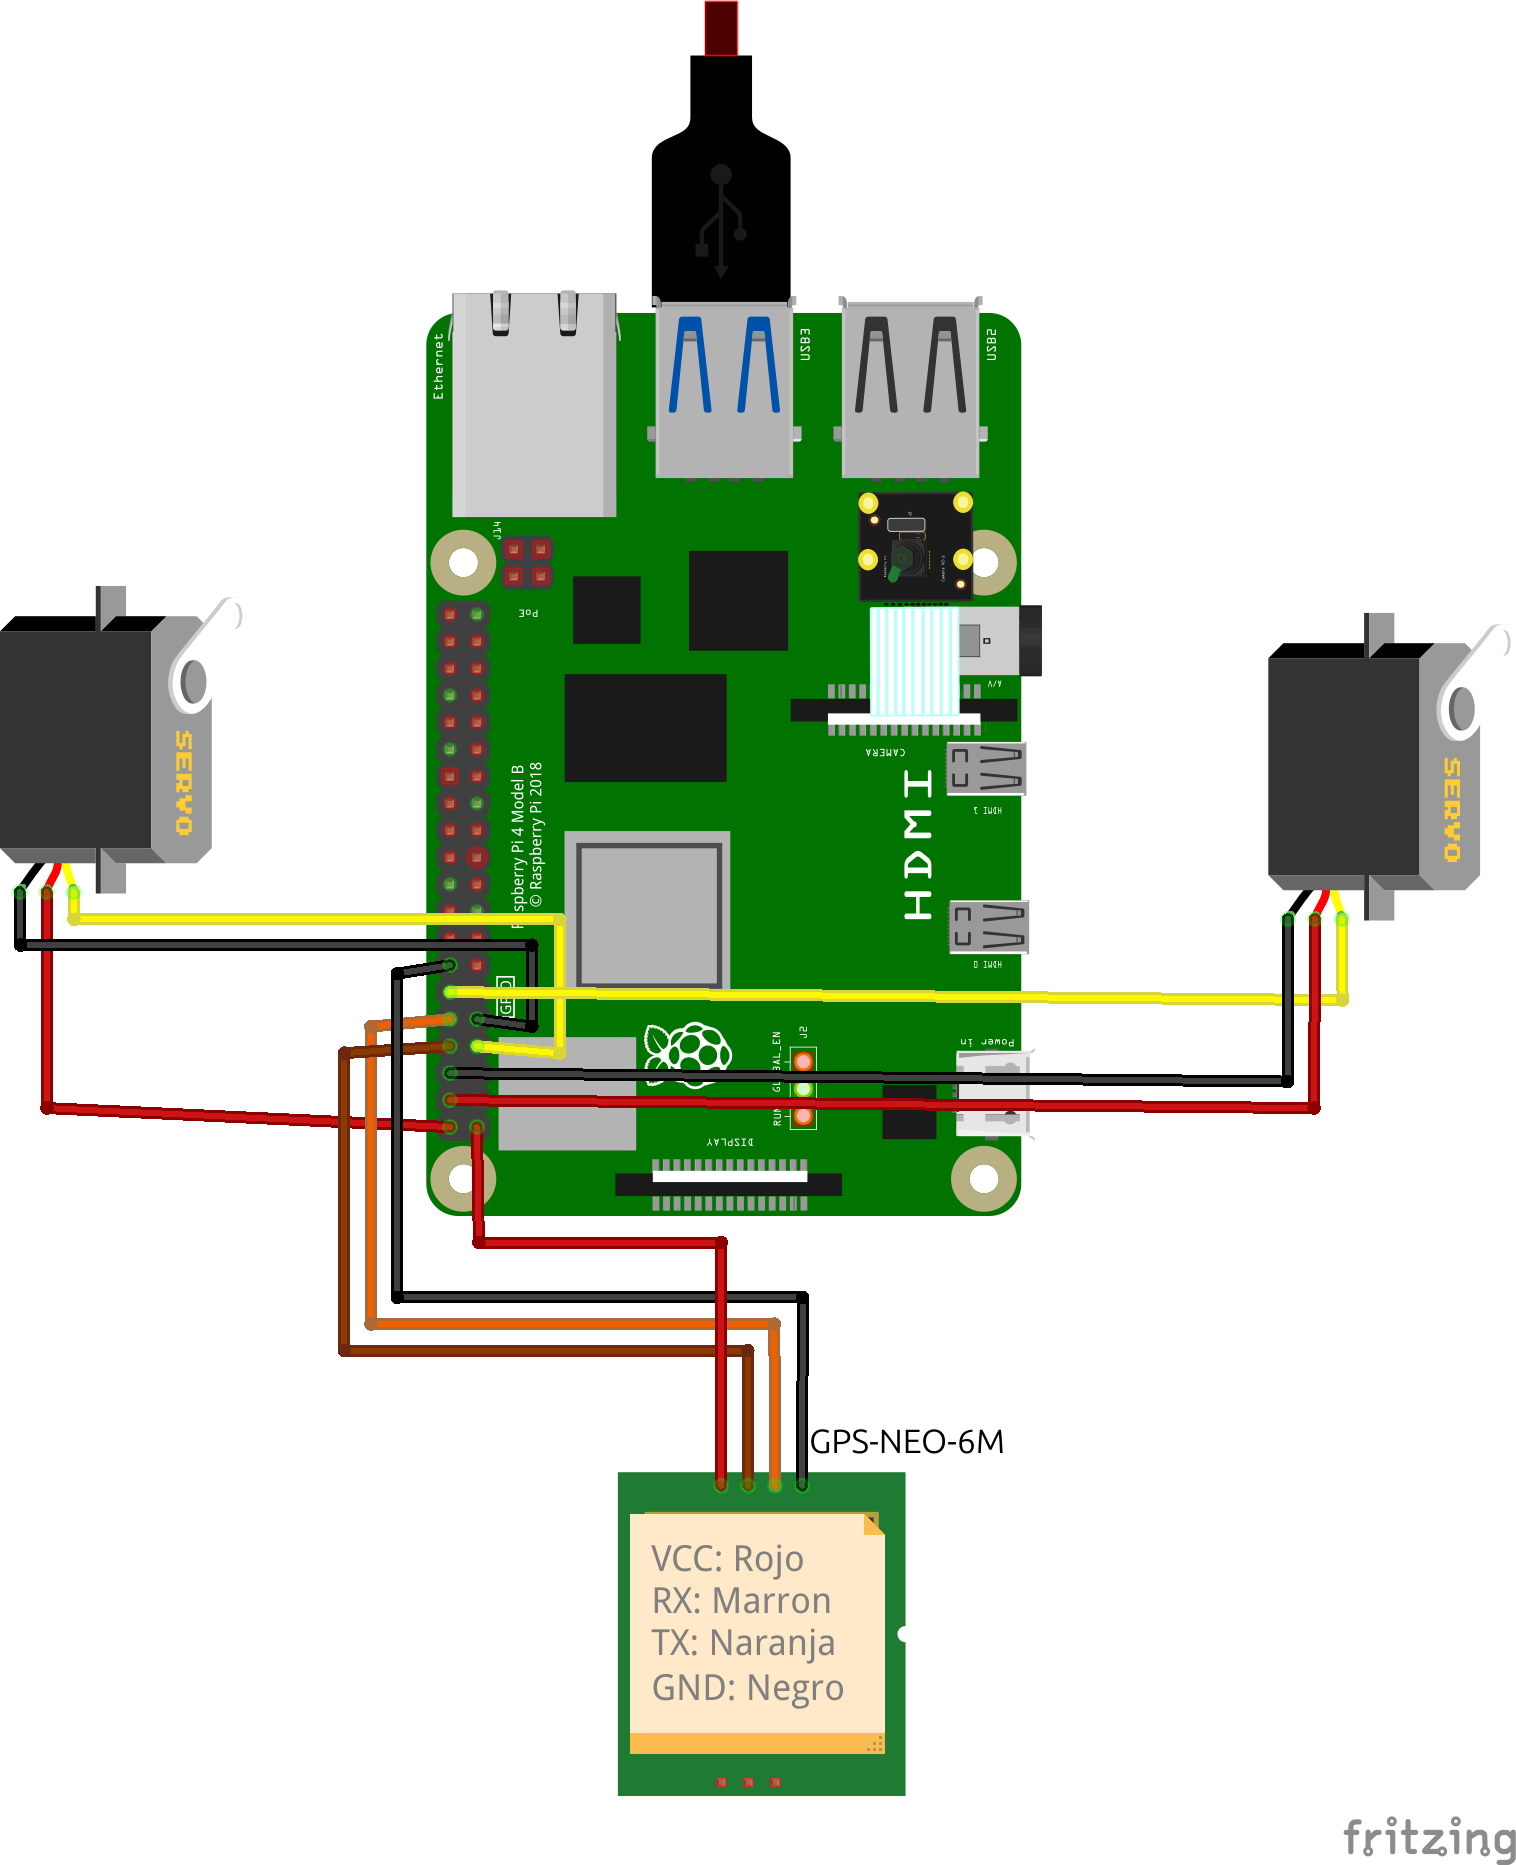
\includegraphics[width=0.8\textwidth]{figs/modelocompleto_bb3.png} \\[5pt]
		\end{column}
	\end{columns}

\end{frame}

\begin{frame}
	\frametitle{Bocetos, maquetas y planos}
	\begin{center}
		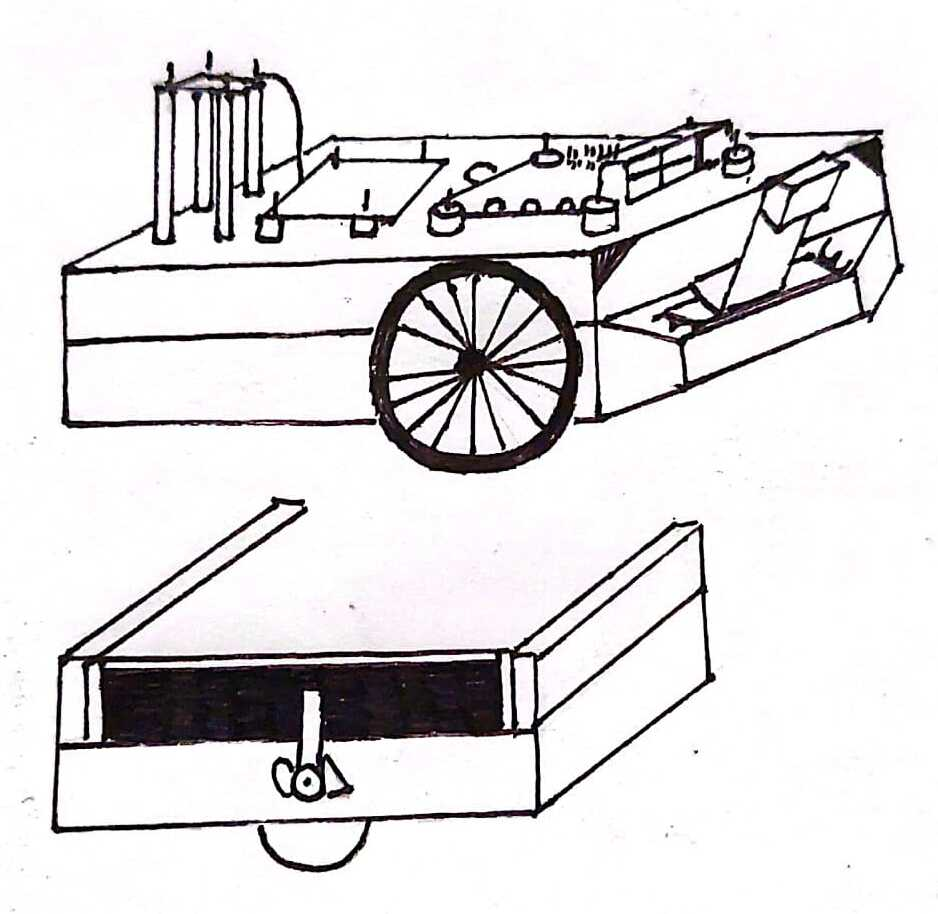
\includegraphics[width=0.2\textwidth]{figs/boceto_papel.jpeg} \hspace{0.5cm}
		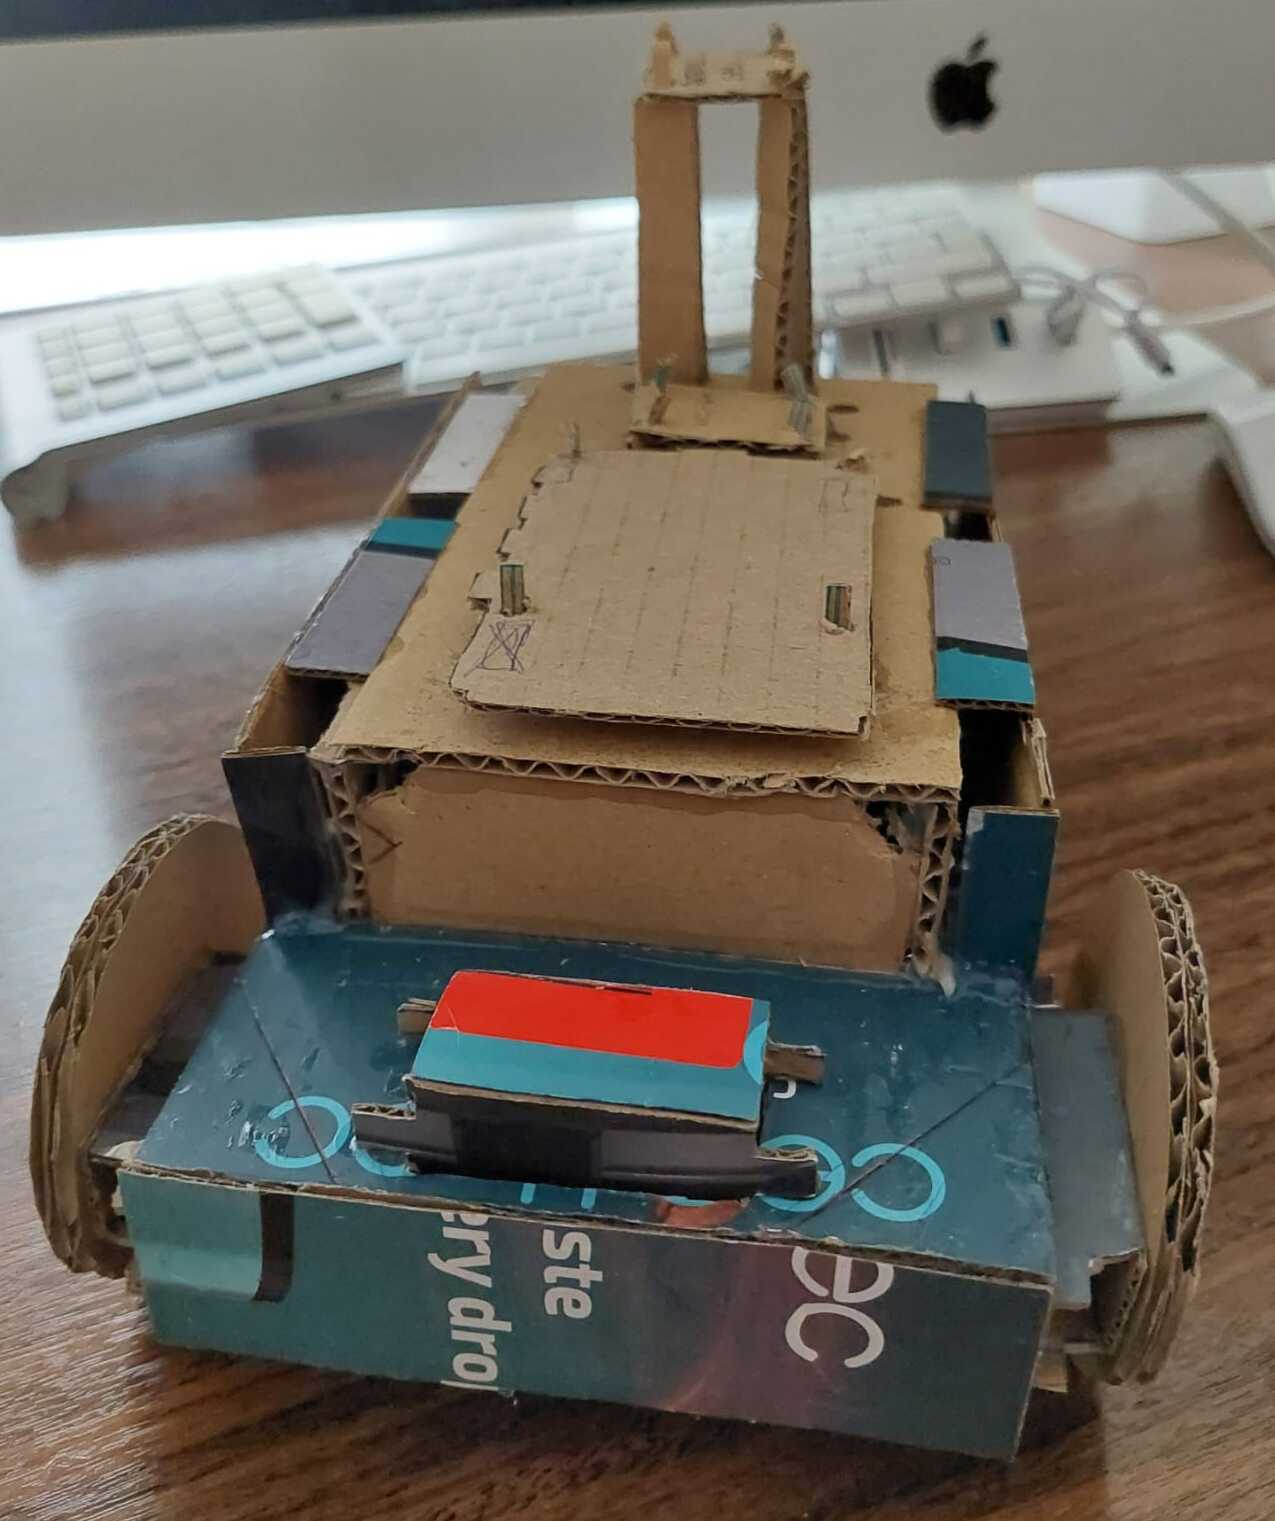
\includegraphics[width=0.2\textwidth]{figs/boceto_carton5.jpeg}
	\end{center}

	\vspace{0.5cm}  % Espacio entre las imágenes de arriba y las de abajo
	\begin{columns}
		% Columna izquierda
		\begin{column}{0.25\textwidth}
			\centering
			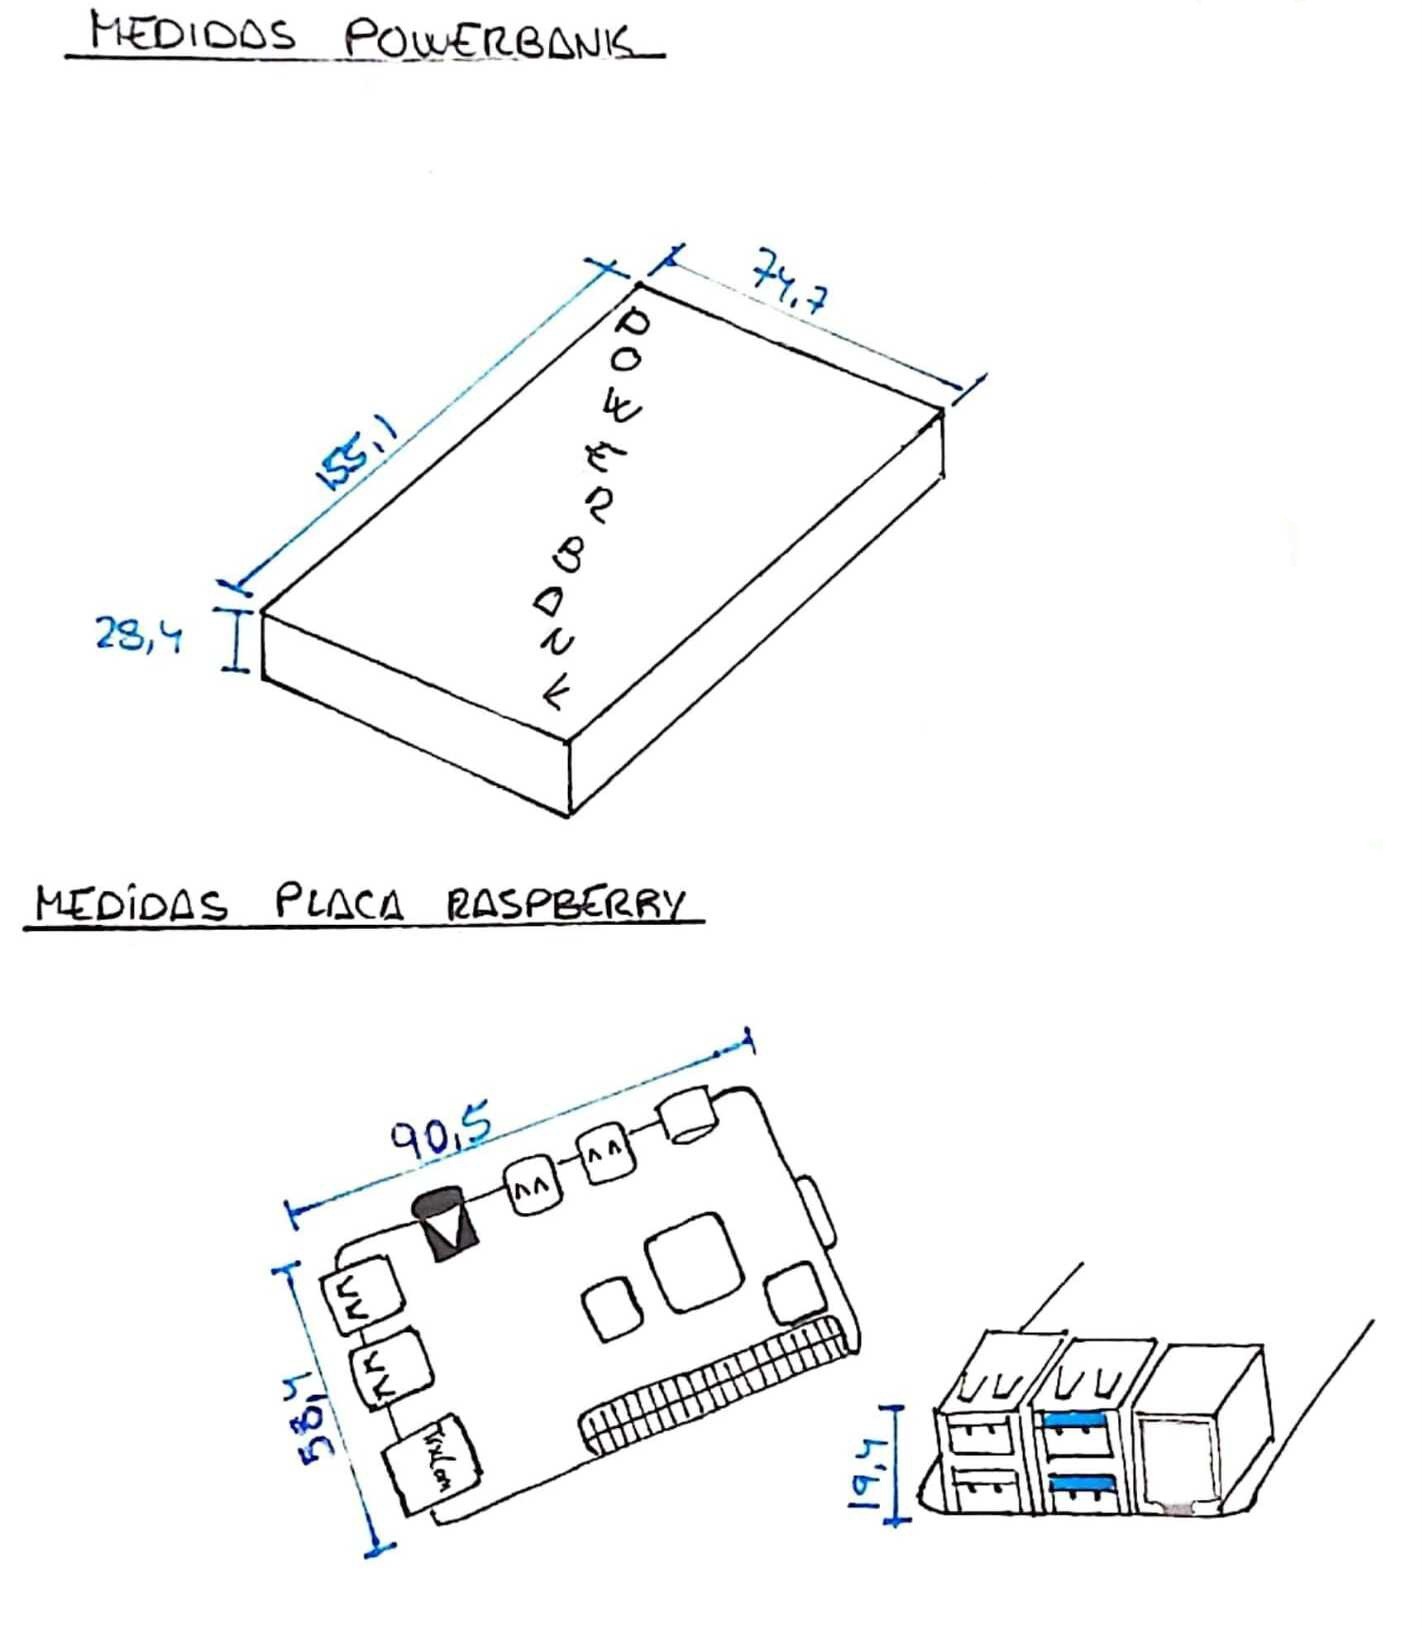
\includegraphics[width=0.8\textwidth]{figs/planos1.jpeg} \\[5pt]
		\end{column}
		% Columna izquierda
		\begin{column}{0.25\textwidth}
			\centering
			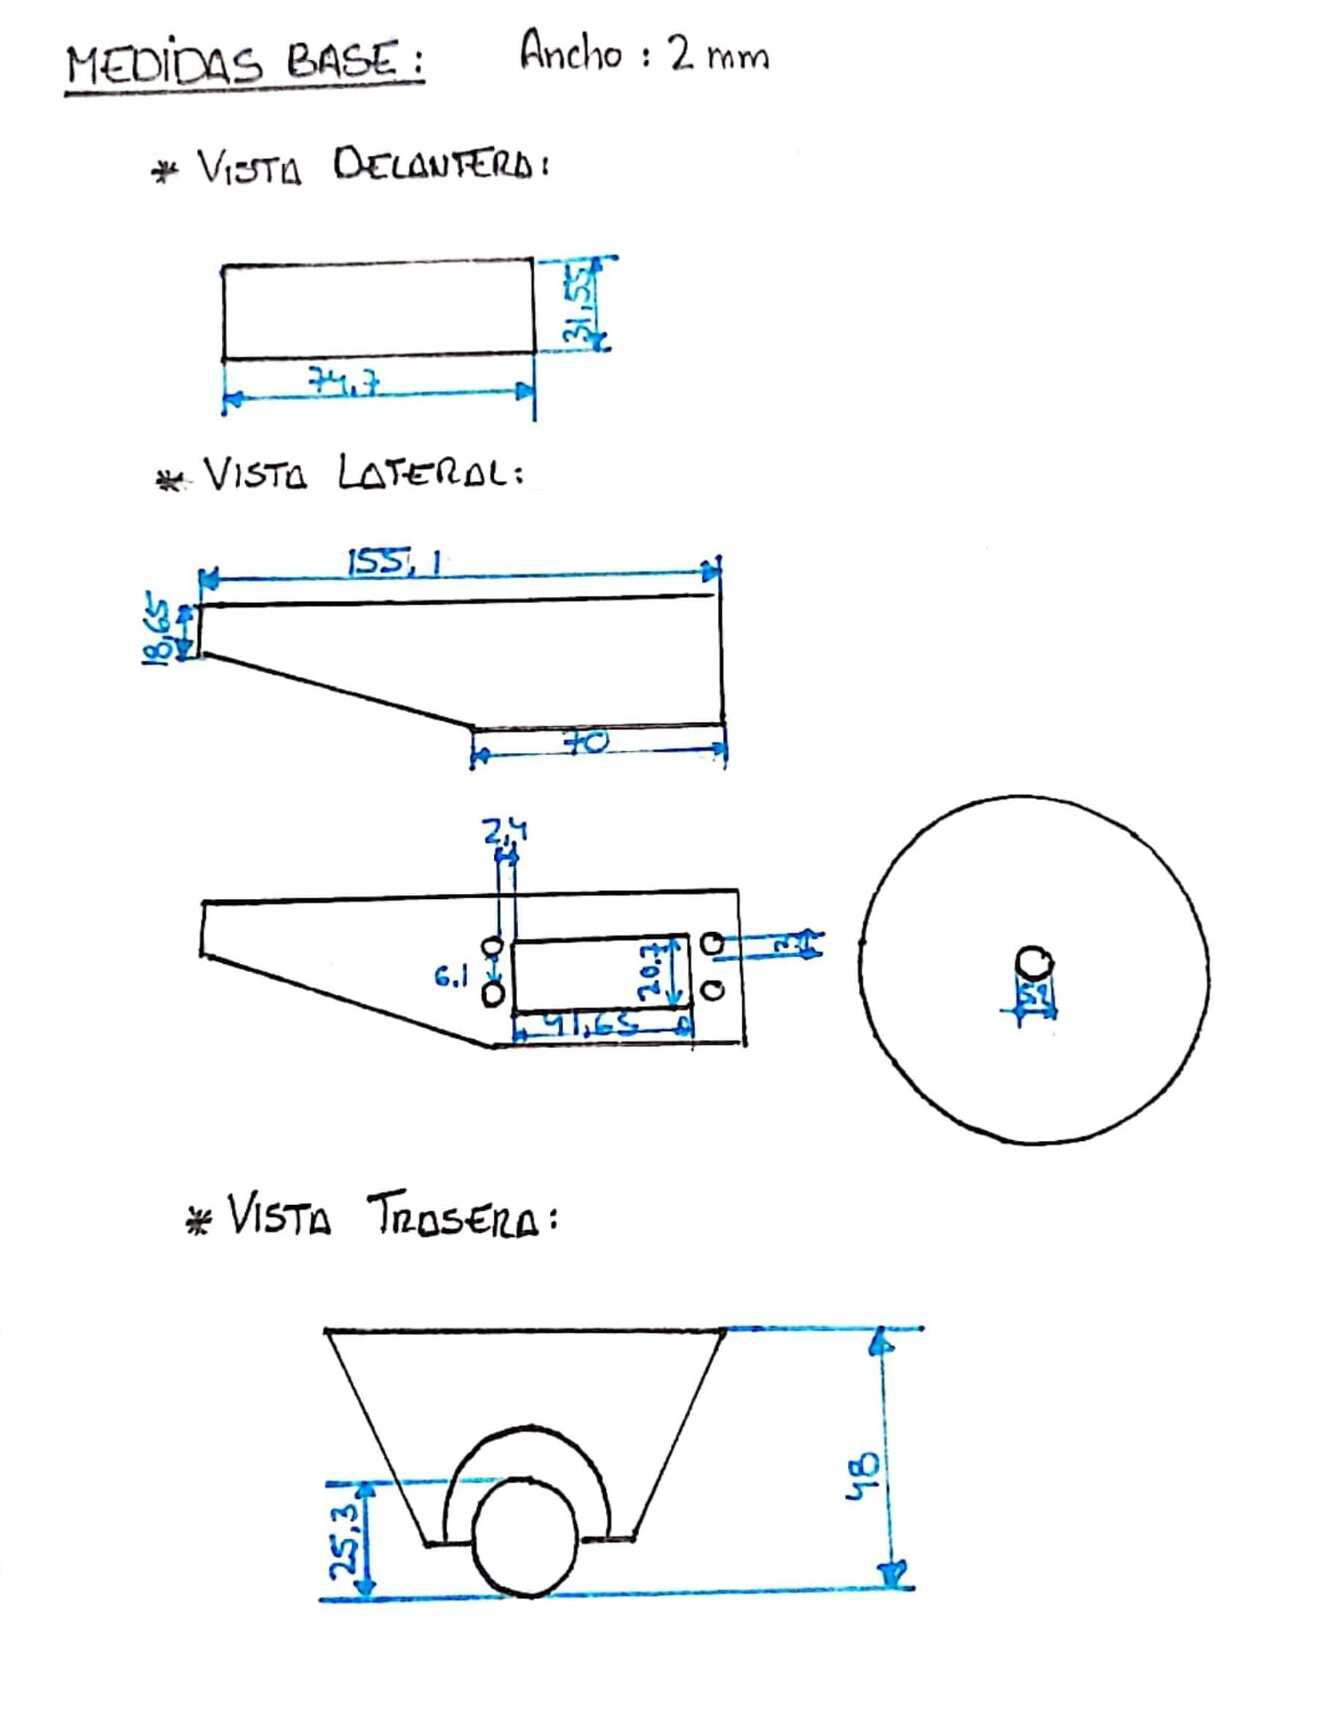
\includegraphics[width=0.8\textwidth]{figs/planos2.jpeg} \\[5pt]
		\end{column}
		% Columna izquierda
		\begin{column}{0.25\textwidth}
			\centering
			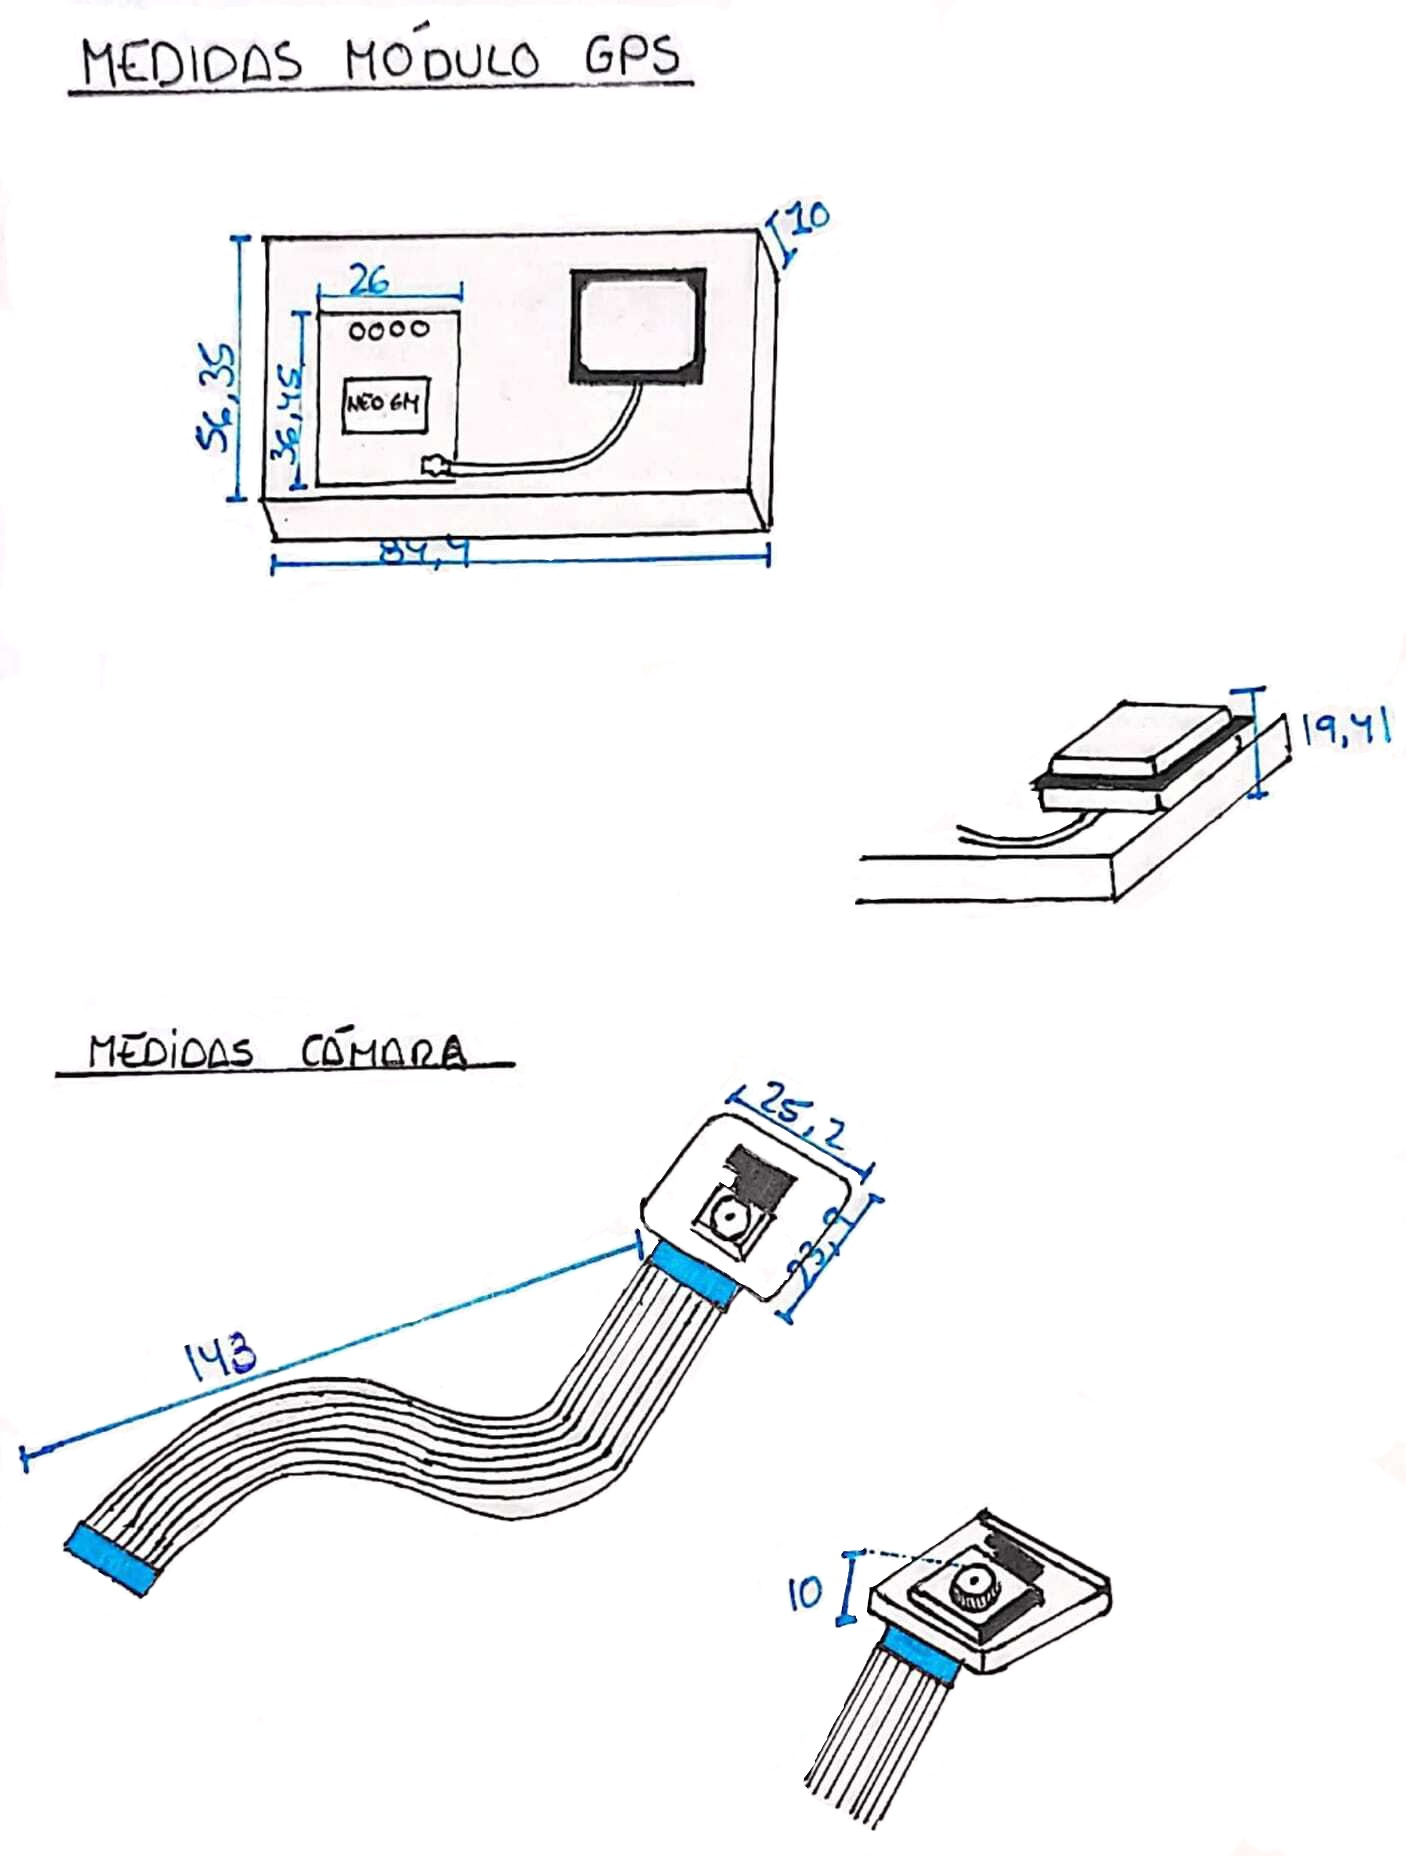
\includegraphics[width=0.8\textwidth]{figs/planos3.jpeg} \\[5pt]
		\end{column}
		% Columna izquierda
		\begin{column}{0.25\textwidth}
			\centering
			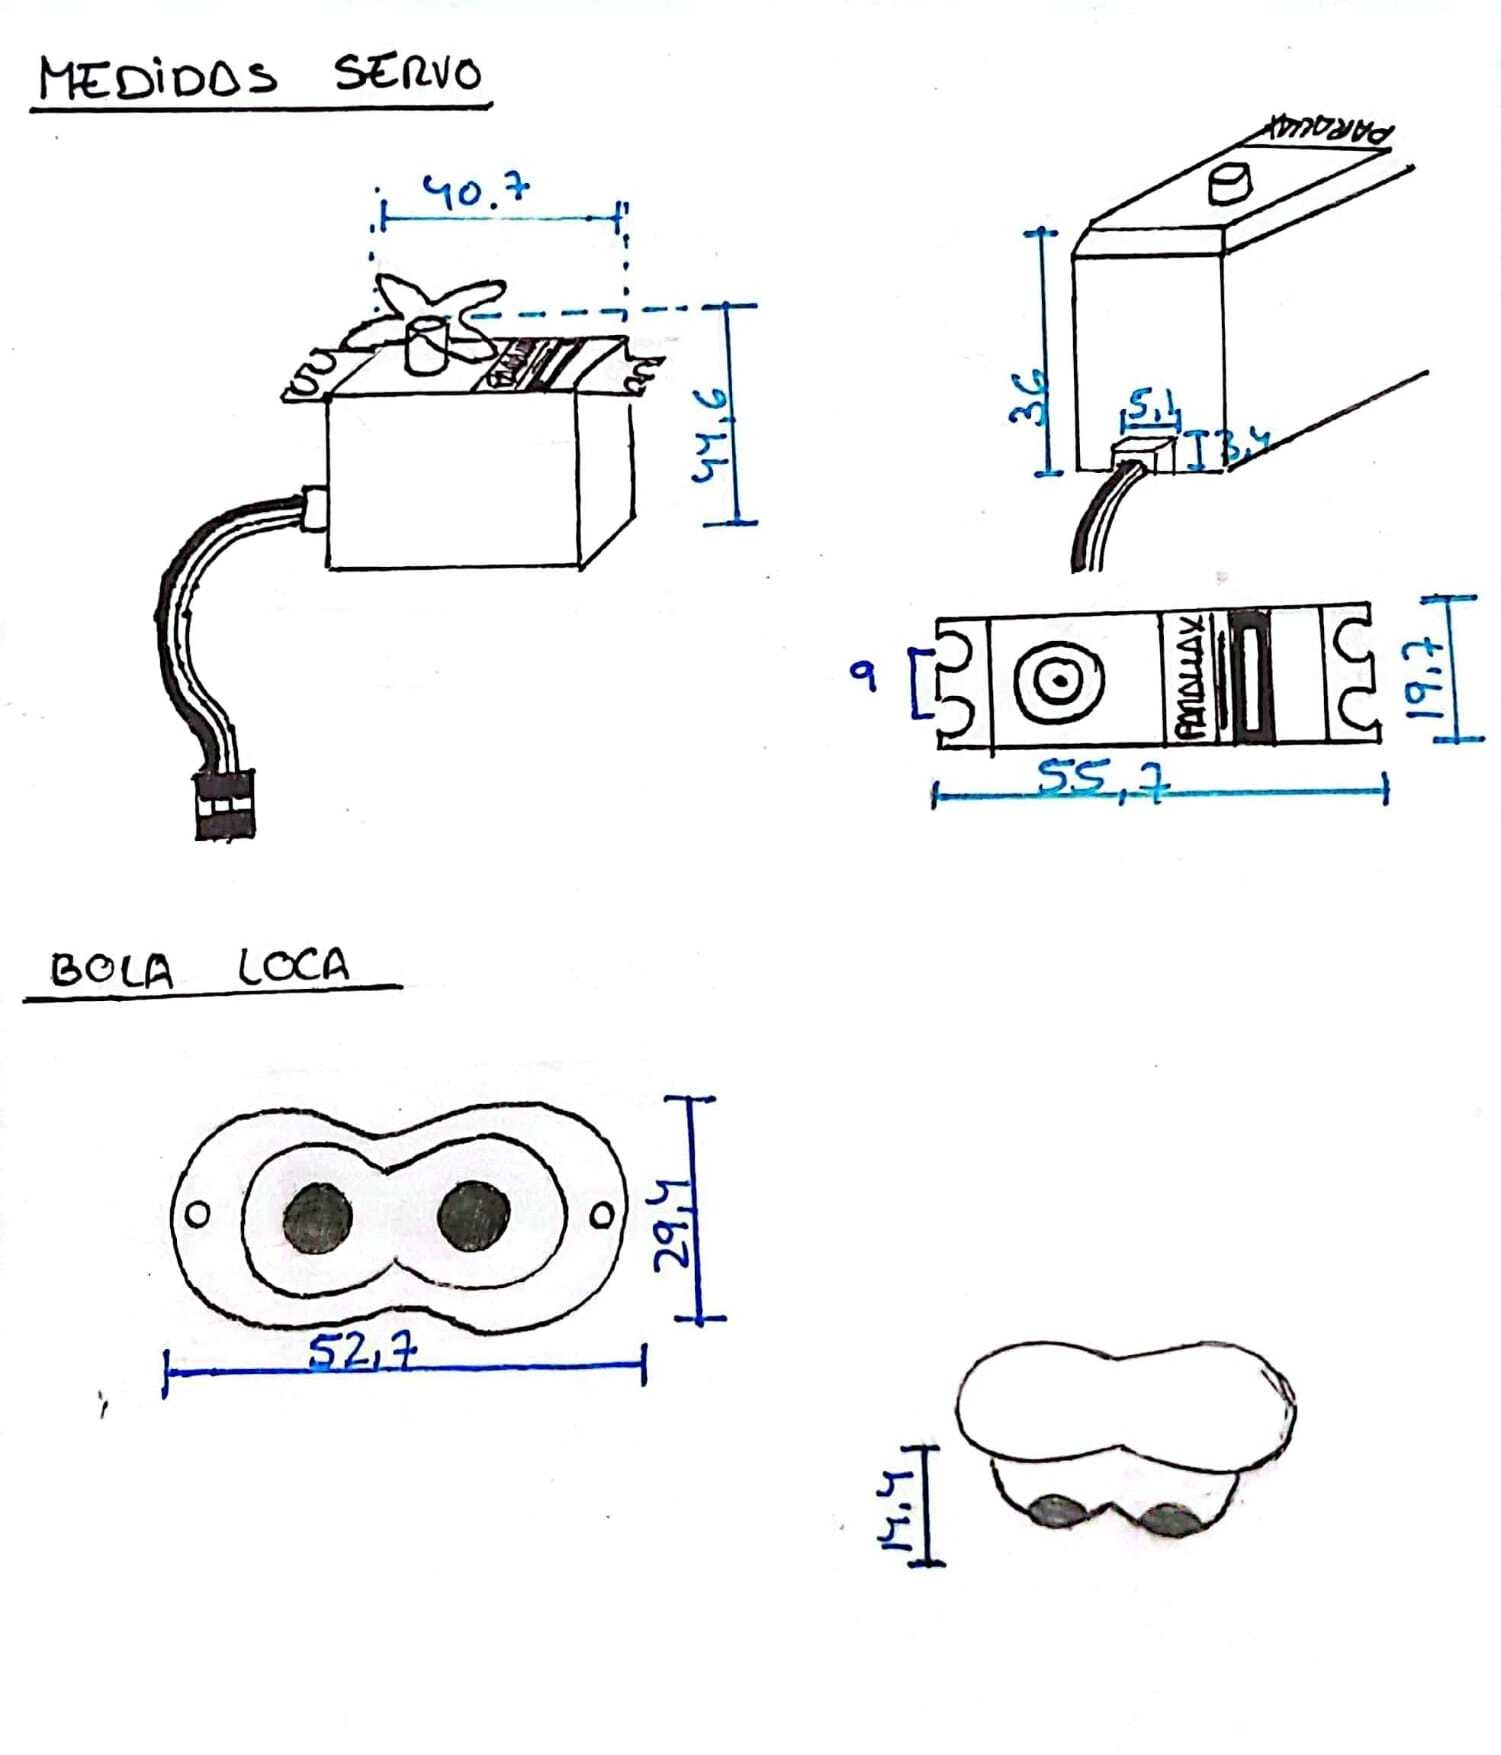
\includegraphics[width=0.8\textwidth]{figs/planos4.jpeg} \\[5pt]
		\end{column}
	\end{columns}
\end{frame}

\begin{frame}
	\frametitle{Piezas diseñadas}
	\begin{columns}
		% Columna izquierda
		\begin{column}{0.5\textwidth}
			\centering
			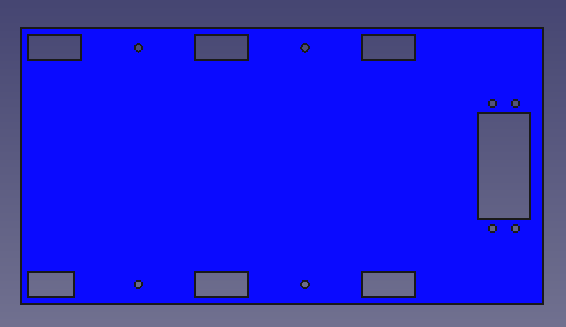
\includegraphics[width=0.87\textwidth]{figs/basevistasuperiorsin.png} \\[20pt]
			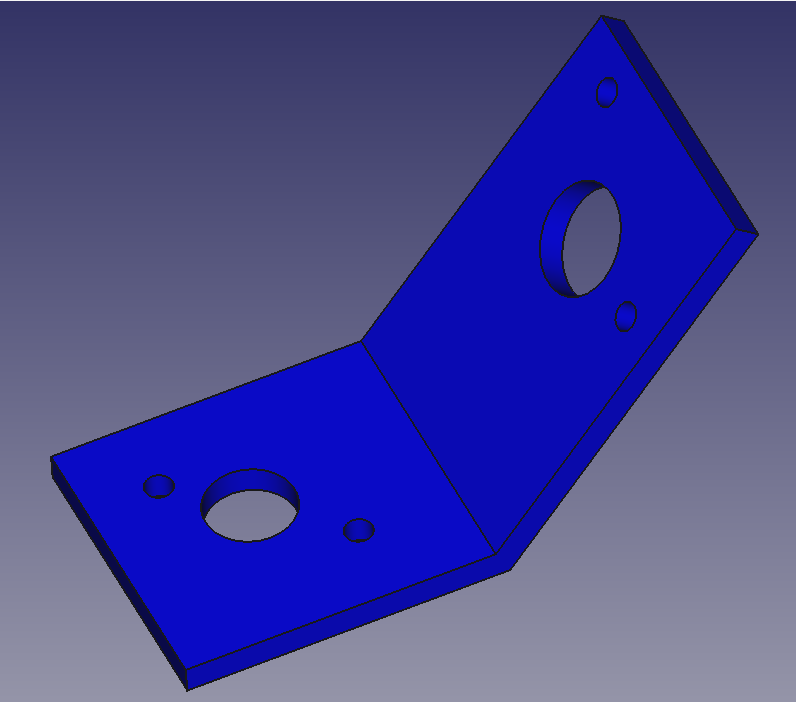
\includegraphics[width=0.5\textwidth]{figs/camera3sin.png}\\[10pt]
		\end{column}
		% Columna izquierdacamera3sin
		\begin{column}{0.5\textwidth}
			\centering
			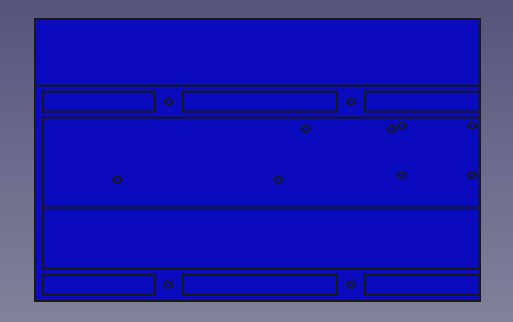
\includegraphics[width=0.8\textwidth]{figs/superior2.png} \\[20pt]
			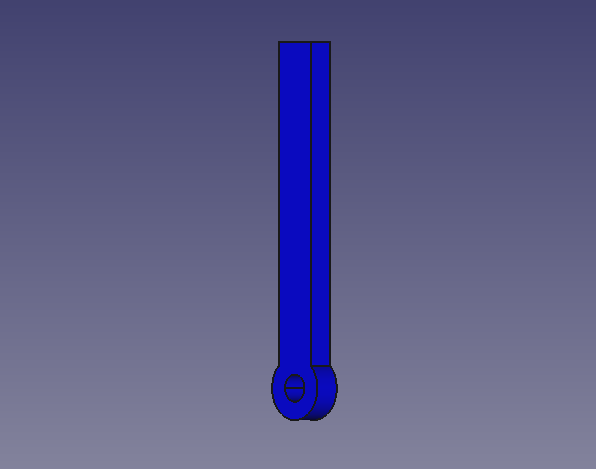
\includegraphics[width=0.55\textwidth]{figs/trasera2.png} \\[10pt]
		\end{column}
	\end{columns}
\end{frame}

\begin{frame}
	\frametitle{Impresión y montaje}
	\begin{figure}
		\centering
		\begin{tabular}{ccc} % 3 columnas
			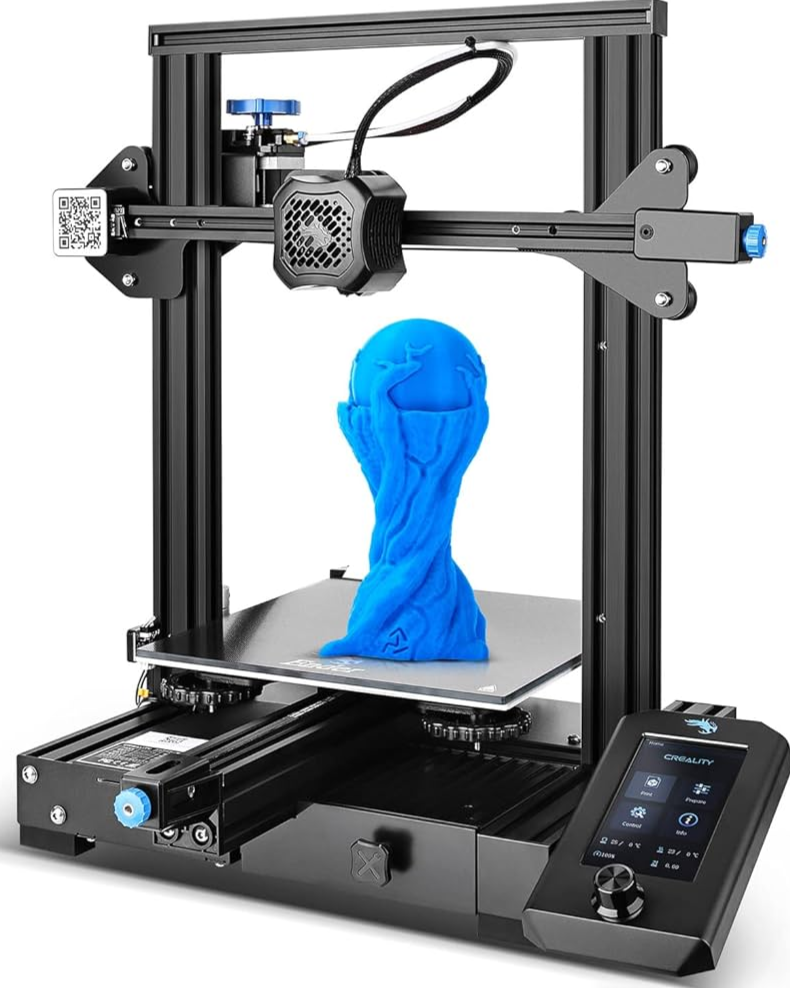
\includegraphics[width=0.18\textwidth]{figs/impresora.jpg} & 
			\includegraphics[width=0.31\textwidth]{figs/setcompleto.jpeg} & 
			\includegraphics[width=0.34\textwidth]{figs/completo3.png} \\[10pt]
			\includegraphics[width=0.23\textwidth]{figs/soldar.jpeg} & 
			\includegraphics[height=0.31\textwidth]{figs/ab.jpeg} & 
			\includegraphics[height=0.31\textwidth]{figs/ra.jpeg}		
		\end{tabular}
	\end{figure}
\end{frame}




%===================================================================================

%============= Soporte software del robot ==========================================
\section*{}
\begin{frame}{}
	\centering \Huge
	\emph{Soporte software del robot}
	\note[item]{Pasemos ahora a comentar los objetivos que nos hemos enfrentado con este trabajo.}
\end{frame}

\section{Soporte software del robot}
% Título en azul (pequeñito) 
\subsection{Simulación}
\begin{frame}
	\frametitle{Simulación}
	% Parte superior con 2 imágenes centradas
	\begin{center}
		\includegraphics[width=0.6\textwidth]{figs/rsp.png} 
	\end{center}
	
	\vspace{0.5cm}  % Espacio entre las imágenes de arriba y las de abajo
	
	% Parte inferior con 1 imagen a la izquierda y 2 imágenes una debajo de otra a la derecha
	\begin{center}
		\begin{columns}
			% Columna izquierda
			\begin{column}{0.5\textwidth}
				\centering
				\includegraphics[width=0.55\textwidth]{figs/rotder.png}
			\end{column}
			% Columna derecha
			\begin{column}{0.5\textwidth}
				\centering
				\includegraphics[width=0.8\textwidth]{figs/rqtimage.png}
			\end{column}
		\end{columns}
	\end{center}
\end{frame}

% Título en azul (pequeñito) 
\subsection{Configuración del robot real}

\begin{frame}
	\frametitle{Configuración del robot real}
	
	\centering
	% Primera fila: ecuación y dos imágenes
	\begin{minipage}{0.35\textwidth}
		\centering
		\begin{equation*}
			\begin{bmatrix}
				497.66 & 0 & 325.3 \\
				0 & 502.16 & 240.18 \\
				0 & 0 & 1 \\
			\end{bmatrix}
		\end{equation*}
	\end{minipage}
	\hspace{0.5cm} % Espacio horizontal entre la ecuación y la primera imagen
	\begin{minipage}{0.2\textwidth}
		\centering
		\includegraphics[width=\textwidth]{figs/traslacion.jpeg}
	\end{minipage}
	\hspace{0.5cm} % Espacio horizontal entre la ecuación y la primera imagen
	\begin{minipage}{0.25\textwidth}
		\centering
		\includegraphics[width=\textwidth]{figs/rotation.jpeg}
	\end{minipage}
	
	\vspace{0.5cm} % Espacio entre las filas
	
	% Segunda fila: dos imágenes centradas
	\begin{minipage}{0.3\textwidth}
		\centering
		\includegraphics[width=\textwidth]{figs/motorlogic1.png}
	\end{minipage}
	\begin{minipage}{0.3\textwidth}
		\centering
		\includegraphics[width=\textwidth]{figs/motorlogic2.png}
	\end{minipage}
	
\end{frame}

% Título en azul (pequeñito) 
\subsection{Comportamiento del robot real}
\begin{frame}
	\frametitle{Detección y obtención del contorno del bache}
	\centering
	\begin{columns}
		% Columna izquierda
		\begin{column}{0.60\textwidth}
			\centering
			\includegraphics[width=0.8\textwidth]{figs/train_results.jpg} \\[5pt]
			\href{https://www.youtube.com/watch?v=Gnwciv4pWf0}{Vídeo de la demostración}
		\end{column}
		% Columna derecha
		\begin{column}{0.4\textwidth}
			\centering
			\includegraphics[height=0.7\textwidth]{figs/contornobache1.png} \\[10pt]
			\includegraphics[height=0.7\textwidth]{figs/contornobache2.png} \\[5pt]

		\end{column}
	\end{columns}
\end{frame}


\begin{frame}
	\frametitle{Modelo de cámara pinhole}
	
	\centering
	% Imagen superior
	\begin{minipage}{0.5\textwidth}
		\centering
		\includegraphics[width=\textwidth]{figs/esquema_pinhole_matrices.jpg}
	\end{minipage}
	
	%\vspace{0.5cm} % Espacio entre las imágenes
	
	% Imagen inferior
	\begin{minipage}{0.5\textwidth}
		\centering
		\includegraphics[width=\textwidth]{figs/pinholecoordinates.png}
	\end{minipage}
	
\end{frame}


\begin{frame}
	\frametitle{Hipótesis suelo}
	\begin{figure}
		\centering
		\includegraphics[width=10cm]{figs/hipotesissuelo.png}
	\end{figure}
\end{frame}

\begin{frame}
	\frametitle{Algoritmo de la lazada}
	%\begin{minipage}{0.5\textwidth}
	\centering
	\begin{equation*}
		A = \frac{1}{2}\abs{\sum_{i=1}^{n-1}x_i y_{i+1} + x_n y_1 - \sum_{i=1}^{n-1}x_{i+1} y_{i} - x_1 y_n}
	\end{equation*}

	Donde $A$ es el área del polígono, $n$ es el número de lados del polígono y $(x_i, y_i)$ , i = 1,2,...,n son los vértices del polígono de forma alternativa.\\[10pt]
	\raggedright Ejemplo teórico: 
	\begin{figure}
		\centering
		\includegraphics[width=8cm]{figs/demoshoelace.png}
	\end{figure}
	%\end{minipage}
\end{frame}

\begin{frame}
	\frametitle{Interfaz web}
	\begin{figure}
		\centering
		\includegraphics[width=11cm]{figs/interfazweb.png}
	\end{figure}
\end{frame}

\begin{frame}
	\frametitle{Detección de líneas}
	\begin{figure}
		\centering
		\includegraphics[width=11cm]{figs/casosdlines.png}
	\end{figure}
\end{frame}

\begin{frame}
	\frametitle{VFF}
	\begin{figure}
		\centering
		\includegraphics[width=5cm]{figs/vff.png}
	\end{figure}
	
\end{frame}
%===================================================================================
%========================== Experimentos ===========================================
\section*{}
\begin{frame}{}
	\centering \Huge
	\emph{Experimentos}
	\note[item]{Pasemos ahora a comentar los objetivos que nos hemos enfrentado con este trabajo.}
\end{frame}

\section{Experimentos}
% Título en azul (pequeñito) 
\subsection{Aplicaciones completas}
\begin{frame}
\frametitle{Teleoperado}
  
  	\begin{figure}
	\centering
	\includegraphics[width=0.5\textwidth]{figs/esquema_nodos_teleoperado_ampliado.png} % Cambia "imagen1.jpg" al nombre de tu imagen
	\end{figure}

\vspace{0.15cm} % Espacio entre las imágenes

\begin{figure}
	\centering
	\includegraphics[width=0.5\textwidth]{figs/teleop_final.png} % Cambia "imagen2.jpg" al nombre de tu imagen
\end{figure}
\end{frame}

\begin{frame}
	\frametitle{Autónomo}
	
	\begin{figure}
		\centering
		\includegraphics[width=0.5\textwidth]{figs/esquema_nodos_vff_ampliado.png} % Cambia "imagen1.jpg" al nombre de tu imagen
	\end{figure}
	
	\vspace{0.15cm} % Espacio entre las imágenes
	
	\begin{figure}
		\centering
		\includegraphics[width=0.5\textwidth]{figs/autonomo_final.png} % Cambia "imagen2.jpg" al nombre de tu imagen
	\end{figure}
\end{frame}


%===================================================================================
%============================= Conclusiones ========================================
\section*{}
\begin{frame}{}
  \centering \Huge
  \emph{Conclusiones}
\note[item]{Para acabar esta presentación, vamos a repasar lo hecho, unas breves conclusiones y las líneas futuras.}
\end{frame}

\section{Conclusiones}
\begin{frame}
\frametitle{Habilidades desarrolladas}
%\begin{block}{Habilidades desarrolladas}
\begin{itemize}
\item FreeCAD.
\item Mecánica y ensamblaje de piezas.
\item Crear un robot en simulación.
\item ROS 2 Control.
\item Modelo de aprendizaje supervisado en una Raspberry Pi.
\item Integración de ROS 2 con páginas web.
\item Generar documentación de calidad en LaTeX.
\end{itemize}
%\end{block}
\end{frame}
	

\begin{frame}
%\begin{block}{Líneas futuras}
\frametitle{Líneas futuras}
\begin{itemize}
\item Soporte software al robot en simulación.
\item Integrar el motor de la cámara.
\item Modificar la altura cámara.
\item Mantener a PiBotJ en la última versión.
\item Implantar una versión más robusta de PiBotJ como un asistente real.
\end{itemize}
%\end{block}
\end{frame}

\begin{frame}[plain]
\large{\titlepage}
\note[item]{Y hasta aquí mi exposición.}
\note[item]{Quedo a disposición del tribunal...}
\end{frame}


%========= Diapositiva con ítems resaltados con colores:
%\begin{frame}
%	\frametitle{Situación de la Robótica}
%	\begin{itemize}
%		\item La \textcolor{red}{tecnología} está cada vez más presente en la vida cotidiana.
%		\item Los robots de servicio aparecen en el \textcolor{blue}{mercado}.
%		\item La \textcolor{red}{domótica} presenta cada vez más aplicaciones domésticas.
%	\end{itemize}
%\end{frame}

%\subsection{Contexto específico}
%========= Diapositiva con bloques:
%\begin{frame}
%	\frametitle{Precedentes de la robótica}
%	\begin{block}{Primera revolución industrial de 1800}
%		Productos fabricados por \textcolor{blue}{máquinas}. La \textcolor{red}{máquina de vapor} fue clave.
%	\end{block}
%\end{frame}


%========= Diapositiva con bullets en diferentes niveles (outline):
%\section{Principios de transducción}
%\subsection{Principio de transducción piezoresistivo}
%\begin{frame}
%\frametitle{Conceptos}
%\begin{outline}
%\1 Piezoresistividad: relación entre resistencia eléctrica y deformación.
%\2 Material piezoresistivo: (1) material en reposo (átomos en equilibrio).
%\3 (2) Si sufre deformación, movimiento átomos, modifican su resistividad.
%\2 Resistencia vs. resistividad de un material.
%\3 Resistencia: depende del volumen del material a tratar.
%\3 Resistividad: caract. intrínseca relacionada con colocación de átomos.
%\end{outline}
%\end{frame}


%\section{Plataforma de desarrollo}
%========= Diapositiva con matemáticas:
%\subsection{Matemáticas empleadas}
%\begin{frame}
%	\frametitle{Matrices de la cámara}
%	\begin{itemize}
%		\item Se usa una matriz $RT (4x4)$ en lugar de $R$ y $T$.
%		\item La matriz $RT$ rota $\theta$ grados en los ejes $X$, $Y$ y $Z$:
%	\end{itemize}
%	\begin{equation}
%		\begin{bmatrix}
%			1 & 0 & 0 & X \\
%			0 & cos(\theta) & sin(\theta) &	Y \\
%			0 & -sin(\theta)& cos(\theta) & Z \\
%			0 & 0 & 0 & 1 
%		\end{bmatrix}
%	\end{equation}
%\end{frame}

%========= Diapositiva con matemáticas y leyenda (conditions*):
%\begin{frame}
%	\frametitle{Resistencia de un material}
%	\begin{outline}
%		\1 Si material piezoresistivo se deforma, cambia su resistencia eléctrica.
%		\begin{equation}
%			R=\rho\frac{l}{A}
%		\end{equation}
%		donde:
%		\begin{conditions*}
%			R & resistencia del material $[\Omega]$\\
%			\rho & resistividad $[\Omega-m]$\\
%			l & longitud $[m]$\\
%			A & área de sección transversal $[m^2]$
%		\end{conditions*}
%		\1 El cambio de resistencia se obtiene a partir de:
%		\begin{equation}
%			\frac{\Delta R}{R}=\frac{\Delta\rho}{\rho}=\frac{\Delta A}{A}=\frac{\Delta l}{l}
%		\end{equation}
%		\1 Otra forma de medir el efecto piezoresistivo: el factor de deformación.
%		\begin{equation}
%			GF(\textit{Gauge Factor})=\frac{\frac{\Delta R}{R}}{\varepsilon}=\frac{\frac{\Delta R}{R}}{\frac{\Delta l}{l}}
%		\end{equation}
%	\end{outline}
%\end{frame}

%========= Diapositiva con códigos:
%\subsection{Algoritmo principal}
%\begin{frame}[fragile]
%	\frametitle{Algoritmo de visión}
%	\begin{lstlisting}
%		cvCvtColor (&image, IplTmp1, CV_RGB2GRAY);//to Gray
%		cvNormalize(IplTmp1, IplTmp1, 0, 255, CV_MINMAX);
%		cvSmooth(IplTmp1,IplTmp2,CV_BLUR,3,3);//Avrg filter
%		cvLaplace(IplTmp2, IplLaplace, 3);//Laplace
%		cvConvertScale(IplLaplace,IplTmp1);
%		cvThreshold(IplTmp1,IplTmp2,Thress,255,CV_THRESH_BIN);
%	\end{lstlisting}
%\end{frame}

\end{document}
